\chapter{Non-Markovian Quantum State Diffusion}
\label{chap:nmqsd}
% * lin/nonlin Markovian SSE
% * little History
% * relevant/irre
%

The description of Markovian open quantum systems in terms of diffusive stochastic differential equations has a long tradition \cite{Ca93_quantum_optics,Pe98_qsd,GaZo04_quantum_noise}.
Especially the related Monte-Carlo methods have become an efficient tool to calculate the time evolution of the system's reduced density operator.
%% ✔ same applies to nmqsd unravelling: \cite{St96_lin_nmqsd}; microscopical theory: ...
%%     => later is described in first section
%% ✔ on its basis we derive a linear \NMSSE, completely equivalent to micro. model, but numerical inferior
%% * key point in hierachy later
%% * interpreation no so clear as markovian case
%% * finite temperature, since derivation depends on vacuum initial bath state
%%
%% * study exemplary system, propose direct solution for T=0
In the present work we are concerned with a generalization of the numerical methods to non-Markovian systems based on the non-Markovian stochastic Schrödinger equation (\NMSSE).
But the latter provides much more than just a favorable unravelling of the reduced density operator:
Actually, it constitutes an equivalent representation of the Schrödinger equation of a full system-environment model without any approximation.
The key to an efficient numerical technique is the Monte-Carlo evaluation of the partial trace over the environmental degrees of freedom to obtain the reduced density operator.

At the beginning, we introduce the standard open-system model, which constitutes the foundation for the rest of this work.
Following the lines of Diósi, Strunz and Gisin \cite{DiSt97_nmsse,DiGiSt98_nmqsd,StDiGi99_nmq_traj}, we derive the linear \NMSSE and demonstrate its connection to the well-known Markovian stochastic Schrödinger equations as well as the usual approach to open quantum systems in terms of Master equations.
The nonlinear version presented in \autoref{sec:nmqsd.nonlin_nmsse} helps to improve the efficiency of the Monte-Carlo evaluation.
\Autoref{sec:nmqsd.interpretation} provides a new pictorial interpretation of the \NMSSE that helps to understand the role of individual interaction-terms.
Since the previous sections crucially rely on the vacuum initial conditions of the environment, we show in \autoref{sec:nmqsd.temperature} how to modify our approach to incorporate an initial thermal state.
This chapter is concluded by an analytic treatment of the Jaynes-Cummings model.

\ref{eq:app.agg_hamil,eq:}
%%%%%%%%%%%%%%%%%%%%%%%%%%%%%%%%%%%%%%%%%%%%%%%%%%%%%%%%%%%%%%%%%%%%%%%%%%%%%%%
\section{The Microscopic Model}
\label{sec:nmqsd.model}
% ✔ standard model (why oscillators, why linear coupling?)
% ✔ reservoir/environment
% ✔ initial states
%
%
%%%%%%%%%%%%%%%%%%%%%%%%%%%%%%%%%%%%%%%%%%%%%%%%%%%%%%%%%%%%%%%%%%%%%%%%%%%%%%%

It is the foremost goal of this work to obtain a dynamical description of an open-system's reduced state.
Nevertheless, we introduce a full model of system and environment first, that is the non-relativistic standard model of an open quantum system coupled to a bosonic environment extensively studied for example in the book of Weiss \cite{We99_dissipative_systems}.
There are three reasons for such a microscopic approach:
On one hand, this serves the purpose to better understand the physical origin of macroscopical properties used to characterize the environment later on.
But more importantly, starting with a closed quantum system is the only strategy allowing us to derive the \NMSSE from first principles, namely the Schrödinger equation.
As a last argument we mention that the reduced dynamics are greatly influenced by the choice of initial conditions.
Especially entanglement between the system and its environment may change the reduced dynamics dramatically \cite{PhysRevA.64.062106}---in what follows we ignore this point and always work with separable initial conditions.\\



As a starting point, we consider an environment consisting of a finite number $N$ of uncoupled harmonic oscillators\footnote{% FOOTNOTE %%%%%
  We use \quotes{environment}, \quotes{reservoir} and \quotes{bath} interchangeably though the latter two suggest a large size compared to the system.
}.
A generalization to an infinite number can be carried out formally along the same lines, replacing sums by infinite series or even integrals; a different approach within our framework is presented later.
The dynamics of both system and environment are then described by a unitary time evolution with Hamiltonian
\begin{equation}
  \Htot = \Hsys \otimes \unit  +  \unit \otimes \Henv  +  \Hint,
  \label{eq:nmqsd.Htot_schr}
\end{equation}
where $\Hsys$ and $\Henv$ are the free Hamiltonians of the system and the bath respectively and $\unit$ denotes the identity on the appropriate Hilbert space.
%\footnote{% FOOTNOTE %%%%%
%  For some models like the damped harmonic oscillator \cite{CaLe83_diss_system} an additional renormalization term arises from the interaction.
%  Nevertheless, such a contribution is attributed to $\Hsys$ since it only acts on the system's Hilbert space.
%}
The latter is a sum over free harmonic oscillators $\Henv = \sum_\lambda \omega_\lambda \adj{a}_\lambda a_\lambda$ expressed in bosonic ladder operators $a_\lambda$ and $\adj{a}_\lambda$ of the $\lambda$\th mode with frequency $\omega_\lambda$.
Treating a finite number of independent reservoirs poses no further difficulties and therefore is not elaborated in this section.

For the interaction between environment and system we confine ourselves to the case of linear coupling
\begin{equation}
  \Hint = \sum_\lambda \cc{g}_\lambda \, L \otimes \adj{a}_\lambda + g_\lambda \, \adj{L} \otimes a_\lambda.
  \label{eq:nmqsd.Hint}
\end{equation}
Here $L$ denotes the coupling operator in the system's Hilbert space and $g_\lambda \in \Complex$ the coupling strength of the $\lambda$\th mode.
In the field of condensed matter physics, typical models involve a coupling of an individual bath mode that scales inversely with the environment size \cite{We99_dissipative_systems}, hence, the linear coupling in~\ref{eq:nmqsd.Hint} seems reasonable for macroscopic large reservoirs.
Also, the interaction of an electron with the electro-magnetic field is described by a Hamiltonian~\ref{eq:nmqsd.Hint} up to very high precision---leaving aside some extreme conditions \cite{WaMi08_quantum_optics}.
But our framework is not restricted to such weak-coupling regimes, therefore, in such cases the linearity is imposed as another assumption.

%% OPEN SYSTEM %%%%%%%%%%%%%%%%%%%%%%%%%%%%%%%%%%%%%%%%%%%%%%%%%%%%%%%%%%%%%%%%%
\begin{figure}
  \centering
  \documentclass{standalone}
\usepackage{amsmath}
\usepackage{tikz}
\usetikzlibrary{matrix}
\usetikzlibrary{calc}
\begin{document}
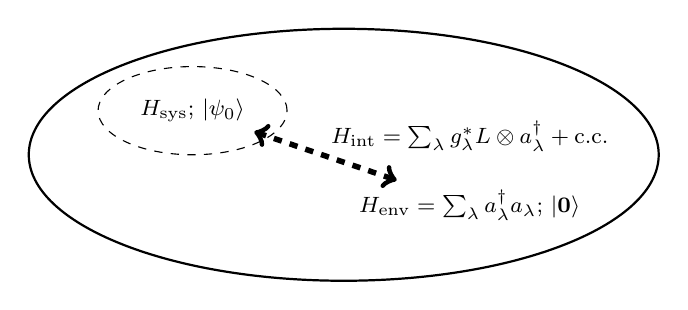
\begin{tikzpicture}[scale=.8]
  \node[align=center] at (-2.4, .7) (sys) {\footnotesize $H_\mathrm{sys}$; $|\psi_0\rangle$};
  \draw[dashed] (-2.4,.7) ellipse (1.5 and .7);
  \node[align=center,] at (2, -.8) (env) {\footnotesize $H_\mathrm{env}=\sum_\lambda a_\lambda^\dagger a_\lambda$;  $|\boldsymbol{0}\rangle$};

  \draw[thick] (0, 0) ellipse (5 and 2);

  \draw[<->, line width=2, dashed] (sys) -- (env);

  \node[align=right] at (2, .3) {\footnotesize $H_\mathrm{int} = \sum_\lambda g_\lambda^* L \otimes a_\lambda^\dagger + \mathrm{c.c.}$};

\end{tikzpicture}
\end{document}

  \caption{%
    Standard model of an open system immersed into a bosonic bath at zero temperature.
    The environmental oscillators with frequencies $\omega_\lambda$ are described in terms of ladder operators $a_\lambda$ and $\adj{a}_\lambda$.
    A coupling operator $L$ mediates the influence of the environment.
  }
  \label{fig:nmqsd.open_system}
\end{figure}
%%%%%%%%%%%%%%%%%%%%%%%%%%%%%%%%%%%%%%%%%%%%%%%%%%%%%%%%%%%%%%%%%%%%%%%%%%%%%%%%

Beside the full Hamiltonian, another important influence on the system's time evolution is the initial state, specifically the initial entanglement between system and bath.
Throughout this work we only consider product initial conditions, where the bath is in the vacuum state with respect to all $a_\lambda$
\begin{equation}
  \ket{\Psi_0} = \ket{\psi_0} \bigotimes\limits_\lambda \ket{0_\lambda}.
  \label{eq:nmqsd.initial_conditions}
\end{equation}
Such a choice is not as restrictive as it seems on first glance: In \autoref{sec:nmqsd.temperature} we show how a thermal bath state can be mapped to this case.
However, it is far from clear if the results of this work carry over to more general initial conditions, as the \NMSSE and most strategies to solve it crucially depend on \autoref{eq:nmqsd.initial_conditions}.\\



To absorb the free dynamics of the environment in time dependent creation and annihilation operators, we switch to the interaction picture with respect to $\Henv$.
Since the bath operators merely obtain an additional phase $\exp[\pm \ii \omega_\lambda t]$, the transformed Hamiltonian from \autoref{eq:nmqsd.Htot_schr} reads\footnote{% FOOTNOTE %%%%%
  We refrain from introducing another label to distinguish between time evolution pictures; in what follows we always work in the interaction picture unless stated otherwise.
}
\begin{equation}
  \Htot(t) = \Hsys \otimes \unit  +  \sum_\lambda \left( \cc{g}_\lambda \exp[\ii \omega_\lambda t] \, L \otimes \adj{a}_\lambda + g_\lambda \exp[-\ii \omega t] \, \adj{L} \otimes a_\lambda \right).
  \label{eq:nmqsd.Htot}
\end{equation}
Our choice of separable initial conditions with a vacuum bath state ensures that the reduced density operator remains unaffected under the change of time evolution picture.

It is instructive to rewrite the last equation using the operator valued \quotes{force}
\begin{equation}
  B(t)=\sum_\lambda g_\lambda a_\lambda \exp[-\ii\omega_\lambda t].
  \label{eq:nmqsd.force_operator}
\end{equation}
The total Hamiltonian then reads $\Htot(t) = \Hsys \otimes \unit  +  L \otimes \adj{B(t)}  +  \adj{L} \otimes B(t)$.
From this equation it can already be seen that the complete action of the environment on the system is encoded in the operator $B(t)$.
An important---and within our model the only---characteristic of the environment is the \emph{two-time correlation function} $\alpha(t-s) = \big\langle  (B(t) + \adj{B(t)})(B(s) + \adj{B(s)}) \big\rangle_\rho$, where $\qmean{\cdot}_\rho$ denotes the expectation value with respect to an arbitrary initial bath density matrix $\rho$.
For a thermal state at temperature $T$, the correlation function can be calculated analytically \cite{FeHi10_path_integrals}
\begin{equation}
  \alpha_T(t - s) = \sum_\lambda  \abs{g_\lambda}^2  \left( \operatorname{coth} \left( \frac{\omega_\lambda}{2T} \right) \, \cos \omega_\lambda (t-s)  -  \ii \sin \omega_\lambda(t-s) \right).
  \label{eq:nmqsd.thermal_correlation_function}
\end{equation}
Introducing the \emph{spectral density} $J(\omega) = \sum_\lambda \abs{g_\lambda}^2 \delta(\omega - \omega_\lambda)$ and taking the limit $T \to 0$, \autoref{eq:nmqsd.thermal_correlation_function} is written more concisely as
\begin{equation}
  \alpha_0(t - s) = \qmean{B(t)\adj{B(s)}}_0 = \int_0^\infty J(\omega) \exp[-\ii\omega (t-s)] \dd \omega,
  \label{eq:nmqsd.correlation_function}
\end{equation}
provided all oscillator-frequencies $\omega_\lambda$ are positive.
In other words, the zero temperature correlation function is simply the (one-sided) Fourier transform of the spectral density.
Since a genuine physical spectral density is real, we require admissible correlation functions to be hermitian $\alpha(-t) = \cc{\alpha(t)}$.

Typical correlation functions of macroscopic systems decay exponentially on a timescale $\tau_\mathrm{c}$ called correlation time.
The Markov limit $\tau_\mathrm{c} \to 0$ amounts to a completely memoryless time evolution and leads to the celebrated quantum dynamical semi-groups.
On the other hand, a finite environment yields a purely oscillatory correlation function with $\tau_\mathrm{c} \to \infty$.

%%%%%%%%%%%%%%%%%%%%%%%%%%%%%%%%%%%%%%%%%%%%%%%%%%%%%%%%%%%%%%%%%%%%%%%%%%%%%%%
\section{Linear NMSSE}
\label{sec:nmqsd.lin_nmsse}
% ✔ Bargman States, hilbert space valued functions
% ✔ derivation
% * problems, non-locality in noise
% ✔ reduced density operator
% * relative state --> interpretation; but also connection with H_s valued functions
% ✔ zero temperature, importance for calculations
% * quantum trajectory Carmichael
%
%%%%%%%%%%%%%%%%%%%%%%%%%%%%%%%%%%%%%%%%%%%%%%%%%%%%%%%%%%%%%%%%%%%%%%%%%%%%%%%

The linear non-Markovian stochastic Schrödinger equation (\NMSSE) derived in this section is an equivalent reformulation of the interaction-picture Schrödinger equation
\begin{equation}
  \partial_t \ket{\Psi_t} = -\ii \Htot(t) \ket{\Psi_t}, \qquad \ket{\Psi_0} = \ket{\psi_0} \otimes \ket{0},
  \label{eq:nmqsd.schroedinger_ia}
\end{equation}
corresponding to the model of the last section.
As we elaborate in this section, expressing the bath degrees of freedom in the Bargmann Hilbert space of anti-holomorphic functions\cite{Ba61_coherent_states} provides a representation well suited to a stochastic interpretation.
To this end, we introduce the unnormalized coherent state $\ket{z_\lambda} = \exp(z_\lambda \adj{a}_\lambda)\ket{0_\lambda}$ for each mode with resolution of the identity for the environment
\begin{equation}
  \unit = \int \frac{\exp[-\abs{\zz}^2]}{\pi^N} \, \ket{\zz}\bra{\zz} \dd^{2N}z.
  \label{eq:nmqsd.identity}
\end{equation}
Here, we employ the shorthand notation $\ket{\zz} = \bigotimes_\lambda \ket{z_\lambda}$ and the \quotes{volume} integration measure for $N$ complex numbers $\dd^{2N}z = \prod_\lambda \dd\Re z_\lambda \dd\Im z_\lambda$.
Throughout this work the finite bath is often replaced by a continuum of oscillators, therefore, we simply write $\mudz = \pi^{-N} \exp(-\abs{\vec z}^2) \dd^{2N}z$ and drop the explicit reference to $N$ to keep notation identical.

\Autoref{eq:nmqsd.identity} allows us to expand the full state in a time-independent environment basis
\begin{equation*}
  \ket{\Psi_t} = \int \ket{\psi_t(\cc\zz)} \otimes \ket{\zz} \mudz.
\end{equation*}
For the following derivation it is crucial to notice that the Bargmann transform $\zz \mapsto \psi_t(\cc\zz)$ is an anti-holomorphic function with values in the system's Hilbert space $\HHsys$.
Naturally, it is equivalent to any other representation of the full state $\ket{\Psi_t}$.
As the coherent states are not orthogonal, but rather satisfy $\braket{\vec w}{\vec z} = \exp(\sum_\lambda \cc w_\lambda z_\lambda)$, the reduced density operator, obtained by tracing over the bath degrees of freedom reads
\begin{equation}
  \rho(t) = \Tr_\mathrm{env} \ket{\Psi_t}\bra{\Psi_t}
          = \int \ket{\psi_t(\cc\zz)}\bra{\psi_t(\cc\zz)} \mudz.
  \label{eq:nmqsd.reduced_matrix}
\end{equation}

% Only Schrödinger equation point of view!
After having established the kinematic structure, the next step is to rewrite the dynamical equation:
The representation of the ladder operators follows from the usual rules $\bra\zz \adj{a}_\lambda = \cc z_\lambda \bra\zz$ and $\bra\zz a_\lambda = \partial_{\cc z_\lambda} \bra\zz$.
These expressions applied to \autoref{eq:nmqsd.schroedinger_ia} yield the system-bath Schrödinger equation in the transformed space
\begin{equation}
  \partial_t \psi_t(\cc\zz) = -\ii\Hsys\psi_t(\cc\zz)  -  \ii L \sum_\lambda \cc g_\lambda \exp[-\ii\omega_\lambda t] \cc z_\lambda \, \psi_t(\cc\zz)  -  \ii \adj{L} \sum_\lambda g_\lambda \exp[\ii\omega_\lambda t] \, \frac{\partial \psi_t}{\partial z_\lambda}(\cc\zz).
  \label{eq:nmqsd.hamiltonian_microsopic}
\end{equation}
Introducing an effective bath operator analogous to \autoref{eq:nmqsd.force_operator}
\begin{equation}
  \ZZ_t(\cc\zz) = - \ii \sum_\lambda \cc g_\lambda \exp[\ii \omega_\lambda t] \cc z_\lambda
  \label{eq:nmqsd.stochastic_process}
\end{equation}
allows us to combine the effect of the first bath-interaction term into a single multiplication operator---or process for reasons explained in the next paragraph.
A similar conversion works for the second term as well with the help of the functional chain rule $\frac{\partial}{\partial \cc z_\lambda} = \int \frac{\partial \ZZ_s}{\partial\cc z_\lambda} \frac{\delta}{\delta \ZZ_s} \dd s$.
Combined, our new equation of motion, the \emph{non-Markovian stochastic Schrödinger equation}, reads \cite{DiGiSt98_nmqsd}
\begin{equation}
  \partial_t \psi_t = -\ii\Hsys\psi_t  +  L\ZZ_t\psi_t  -  \adj{L} \int_0^t \alpha(t-s) \frac{\delta \psi_t}{\delta \ZZ_s} \dd s.
  \label{eq:nmqsd.nmsse}
\end{equation}
As we show in \autoref{sec:nmqsd.interpretation}, the integral boundaries arise by virtue of the initial conditions~\ref{eq:nmqsd.initial_conditions}, but the basic idea is simple:
By definition of our processes~\ref{eq:nmqsd.stochastic_process} an initial state $\ket{\psi_0}\otimes\ket{0}$ translates to an initial $\psi_0$ that is completely independent of the noise.
Then, causality implies that $\psi_t$ can only depend on $\ZZ_s$ for $0 \le s \le t$.\\



Up to this point we have merely rewritten the original Schrödinger equation~\ref{eq:nmqsd.schroedinger_ia} to an equivalent form:
The original system-bath product Hilbert space $\HHsys \otimes \HHenv$ is simply replaced by a Hilbert space of $\HHsys$-valued functions holomorphic in $\cc\zz$.
A different attitude is quite fruitful, especially with a numerical solution of the \NMSSE in mind:
\Autoref{eq:nmqsd.reduced_matrix} can be rewritten as $\rho_t = \E[\ket{\psi_t}\bra{\psi_t}]$, where $\E$ denotes the average over $\mudz = \pi^{-N} \exp(-\abs{\vec z}^2) \dd^{2N}z$.
Put differently, the reduced density matrix $\rho_t$ arises from averaging over stochastic pure state projectors $\ket{\psitz}\bra{\psitz}$ with Gaussian weight $\mudz$.
Hence, we regard \autoref{eq:nmqsd.nmsse} as a stochastic differential equation for individual realizations $\psi_t(\cc\zz)$.
We refer to the latter either as system state relative to $\ket{\zz}$ or, in the spirit of the stochastic Schrödinger equations emerging from continuous measurement theory \cite{Ca93_quantum_optics}, as \emph{quantum trajectory}.

In this approach, the influence of the bath is implemented as a classical stochastic process $\ZZ_t$ defined by the concrete version~\ref{eq:nmqsd.stochastic_process} and the underlying probability measure $\mu$.
It is a complex Gaussian process, uniquely characterized by its expectation value and covariances
\begin{equation}
  \E\,Z_t = 0, \quad \E\,Z_t Z_s =0, \quad\mbox{and}\quad \E\,Z_t \ZZ_s = \alpha(t-s),
  \label{eq:nmqsd.process_properties}
\end{equation}
where $\alpha(t-s)$ is the zero-temperature correlation function~\ref{eq:nmqsd.correlation_function} for $J(\omega) = \sum_\lambda \abs{g_\lambda}^2 \delta(\omega - \omega_\lambda)$.
By virtue of the initial conditions, $\psi_t$ depends on $\cc\zz$ only through the noise process, thus, we can drop the coherent state labels and simply write $\psitZ$ denoting the trajectory corresponding to the realization $\ZZ_t(\cc\zz)$.
To go one step further, we regard \autoref{eq:nmqsd.process_properties} as the defining properties of $\ZZ_t$ without any reference to the microscopic model.
It is this alternative point of view that makes the \NMSSE-approach so powerful.
The entire influence of the environment is encoded in a complex function $\alpha(t)$, which acts both as correlation function for the driving noise $\ZZ_t$ and weight-function under the memory integral.
A generalization to an arbitrary number of bath-oscillators is now straightforward: Simply replacing $\alpha(t)$ by any admissible bath correlation function allows a unified treatment of arbitrary bosonic environments.

Except in the limit $\alpha(t) \propto \delta(t)$, elaborated in \autoref{sub:nmqsd.markov}, the noise process $\ZZ_t$ is correlated for different times.
This non-Markovian behavior, which makes a complete understanding of the dynamics highly desirable for application but also considerably harder, shows up in the equation of motion~\ref{eq:nmqsd.nmsse} as well.
The memory integral contains the functional derivative over the whole timespan and therefore takes the complete history of $\psitZ$ into account.
In its own right the derivative is just as problematic:
Since its computation requires not only the single realization $\ZZ_t$, but in some sense all adjacent ones as well, it seems questionable to regard the \NMSSE~\ref{eq:nmqsd.nmsse} as a genuine stochastic differential equation \cite{GaWi02_real_nmsse}.
Even from the purely pragmatic point of view, both kinds of non-local behavior complicate a direct numerical simulation of the \NMSSE---or even make it completely impracticable.
Nevertheless, there are two quite distinct solutions to this problem as shown in \autoref{sub:nmqsd.lin_nmsse.convolutionless} and \autoref{chap:num}.


%%%%%%%%%%%%%%%%%%%%%%%%%%%%%%%%%%%%%%%%%%%%%%%%%%%%%%%%%%%%%%%%%%%%%%%%%%%%%%%
\subsection{Convolutionless Formulation}
\label{sub:nmqsd.lin_nmsse.convolutionless}
% * on the existence
% * why it solves problems, true stochastic equation
% * dynamics
% * application

As a cure for the non-locality issues, Diósi, Gisin, and Strunz \cite{DiGiSt98_nmqsd} proposed the powerful \emph{$O$-Operator substitution}:
It is based on the additional assumption, that one may replace the functional derivative by a system operator $O(t,s,\ZZ)$, which only depends on the realization of $\ZZ$ itself
\begin{equation}
  \frac{\delta \psi_t(\ZZ)}{\delta \ZZ_s} = O(t, s, \ZZ) \psi_t(\ZZ).
  \label{eq:nmqsd.o_substition}
\end{equation}
Besides getting rid of the derivative, this substitution enables us to rewrite the \NMSSE~\ref{eq:nmqsd.nmsse} in its convolutionless form
\begin{equation}
  \partial_t \psi_t(\ZZ) = -\ii\Hsys\psi_t(\ZZ)  +  L\ZZ_t\psi_t(\ZZ)  -  \adj{L} \bar O(t, \ZZ) \psi_t(\ZZ)
  \label{eq:nmqsd.nmsse_o}
\end{equation}
with the time-local operator
\begin{equation}
  \bar O(t, \ZZ) := \int_0^t \alpha(t - s) O(t, s, \ZZ) \dd s.
  \label{eq:nmqsd.o_bar}
\end{equation}
Conclusively, \autoref{eq:nmqsd.nmsse_o} turns into a genuine stochastic differential equation for the trajectory $\psi_t(\ZZ)$, but in the much smaller Hilbert space of the system.
This makes it exceptionally well suited for dealing with infinite sized environments numerically, provided the $\bar O$-operator is known.
Depending on how accurate we can determine $O(t,s,\ZZ)$, the convolutionless \NMSSE~\ref{eq:nmqsd.nmsse_o} is just as accurate as the original microscopic equation of motion~\ref{eq:nmqsd.schroedinger_ia}.

In general this is done as described below \cite{DiGiSt98_nmqsd}:
From the consistency condition
\begin{equation}
  \partial_t \frac{\delta \psi_t(\ZZ)}{\delta \ZZ_s} = \frac{\delta}{\delta \ZZ_s} \partial_t \psi_t(\ZZ)
  \label{eq:nmqsd.consistency_condition}
\end{equation}
supplied with initial value
\begin{equation}
  O(s, s, \ZZ) = L
  \label{eq:nmqsd.o_initial}
\end{equation}
we derive an equation of motion for $O(t, s, \ZZ)$.
It still contains the functional derivative, but is converted to a system of coupled, deterministic equations using a power series ansatz
\begin{equation}
  O(t, s, \ZZ) = \sum_{n=0}^\infty \int_0^t \dots \int_0^t O_n(t, s, \nu_1, \dots, \nu_n) \dd \nu_1 \dots \dd\nu_n.
  \label{eq:nmqsd.o_series}
\end{equation}
For a few simple systems---for example the Jaynes-Cummings model presented in \autoref{sec:nmqsd.two_level} or its higher dimensional generalizations \cite{JiZhYo12_exact_nmqsd}---an exact analytic expression for $O(t, s, \ZZ)$ is known.
Nevertheless, most treatments rely on approximation schemes, for example a perturbation expansion for small coupling parameters or almost-Markovian environments \cite{YuDiGiSt99_pertubation}.
Also, for an exponential bath correlation function $\alpha(t) = g \exp[-\gamma\abs{t} - \ii\Omega t ]$ (or sums thereof), one can solve the equations of motion for
\begin{equation*}
  \bar O_n(t) := \int_0^t \dots \int_0^t \alpha(t-s) \alpha(t - \nu_1) \ldots \alpha(t - \nu_n) \, O_n(t, s, \nu_1, \dots, \dd\nu_n) \dd \nu_1 \dots \nu_n \dd s
\end{equation*}
numerically.
This yields a coupled set of equations similar to the hierarchy derived in \autoref{sec:num.sheom}.
Setting all $\bar O_n(t) = 0$ for $n > 0$ is referred to as zero order functional expansion or \textsc{ZOFE} \cite{RiRoSt11_fmo,RoStEi11_nmqsd_aggregats}.


%%%%%%%%%%%%%%%%%%%%%%%%%%%%%%%%%%%%%%%%%%%%%%%%%%%%%%%%%%%%%%%%%%%%%%%%%%%%%%%
\subsection{Markov Limit}
\label{sub:nmqsd.markov}
% * markov limit
% * problem with negative energy oscillators
% * relation to lindblad/markovian sse
% * Ito vs Stratonovich
%

Markovian dynamics constitute an important limit in the description of open quantum systems.
In this section we show how a bath correlation function with vanishing correlation time, namely $\alpha(t) = \gamma\delta(t)$, transforms the \NMSSE into the linear, diffusive stochastic Schrödinger equation~\ref{eq:intro.lin_qsd}, thus establishing the link to the well-known Markovian theory.

The vacuum initial conditions $\frac{\delta \psi_0}{\delta \ZZ_s} = 0$ with $s \in \Reals$ imply for an arbitrary bath correlation function
\begin{equation}
  \frac{\delta \psi_t}{\delta \ZZ_t} = \frac{1}{2} \, L \psi_t \qquad (t > 0)
  \label{eq:nmqsd.deriv_psit}
\end{equation}
as we show now directly from the equations of motion\footnote{%% FOOTNOTE %%%%%%
  \Autoref{eq:nmqsd.deriv_psit} deviates from the acquainted result~\ref{eq:nmqsd.o_initial} by a factor $\frac{1}{2}$, as the latter is derived without any reference to the functional derivative and therefore does not account for the singular behavior at $s=t$.
  Instead, the $O$-operator is already introduced in the microscopic model using the Heisenberg time evolution picture for the annihilation operator $a_\lambda$ \cite{St01_habil}.
  Therefore, the substitution \autoref{eq:nmqsd.o_substition} does not hold for $s = t$.
  However, this is insignificant for the integrated operator~\ref{eq:nmqsd.o_bar} as a single point has vanishing weight under the integral.
}.

It is clear from its derivation that the \NMSSE describes a unitary time evolution.
Therefore, it can be solved formally using the Dyson series
\begin{equation}
  \psi_t(\ZZ) = \sum_{n=0}^\infty (-\ii)^n \intl{0}{t}{t_1} \intl{0}{t_1}{t_2} \dots \intl{0}{t_{n-1}}{t_n}  \Htot(t_1) \dots \Htot(t_n) \, \psi_0,
  \label{eq:nmqsd.dyson}
\end{equation}
where $\Htot(t)$ is the reformulation of~\ref{eq:nmqsd.Htot} given by
\begin{equation}
  -\ii \Htot(t) = -\ii \Hsys + L \ZZ_t - \adj{L} \intl{-\infty}{\infty}{s} \alpha(t-s) \frac{\delta}{\delta \ZZ_s}.
  \label{eq:nmqsd.Htot_time}
\end{equation}
Throughout this work we often use the shorthand notation $\adjZZ_t = \int\mathrm{d}s \, \alpha(t-s) \frac{\delta}{\delta \ZZ_s}$ for the last term.
Recall that the bounded integral domain in the \NMSSE arises by virtue of the initial conditions---no such restriction applies to $\adjZZ_t$.

In order to calculate~\ref{eq:nmqsd.deriv_psit}, note that the functional derivative $\frac{\delta}{\delta \ZZ_s}$ of $\Htot(t)$ gives a single contribution $\ii \delta(t - s) L$ due to $\frac{\delta \ZZ_t}{\delta \ZZ_s} = \delta(t - s)$.
This allows us to calculate $\frac{\delta \psi_t}{\delta \ZZ_t}$ order by order in \autoref{eq:nmqsd.dyson}:
With vanishing derivative of $\psi_0$ as imposed by the initial conditions, we obtain for the first order
\begin{equation*}
  \frac{\delta}{\delta\ZZ_t} \intl{0}{t}{t_1} (-\ii) \Htot(t_1) \psi_0 = \intl{0}{t}{t_1} \delta(t - t_1) L \psi_0 = \frac{1}{2} \, L \psi_0
\end{equation*}
and similarly for the second order
\begin{align*}
  \frac{\delta}{\delta\ZZ_t} &\intl{0}{t}{t_1}\intl{0}{t_1}{t_2} (-\ii)^2 \Htot(t_1)\Htot(t_2)\psi_0 \\
  =&\intl{0}{t}{t_1}\intl{0}{t_1}{t_2} (-\ii) \Big( \delta(t - t_1)L \Htot(t_2) + \delta(t - t_2) \Htot(t_1) L \Big)\psi_0 \\
  =& \frac{1}{2}\,L \intl{0}{t}{t_2} (-\ii) \Htot(t_2)\psi_0
\end{align*}
To justify the second identity, notice that $\delta(t - t_2)$ contributes only if $t_1 \ge t$, since otherwise the singular point $t$ of the $\delta$-function lies outside the integration domain.
However, this condition is only satisfied with vanishing weight under the $t_1$ integral, as the latter is confined to $[0,t]$.
The same scheme carries over to all higher orders in \autoref{eq:nmqsd.dyson}, leading to \autoref{eq:nmqsd.deriv_psit}.\\



Now, let us return to the Markov limit of our {\NMSSE}.
By virtue of the singular correlation function $\alpha(t) = \gamma\delta(t)$, the memory integral reduces to a time-local form
\begin{equation*}
  \adjZZ_t = \int \delta(t - s) \frac{\delta}{\delta \ZZ_s}\dd s = \gamma \, \frac{\delta}{\delta \ZZ_t}
\end{equation*}
as it is expected from a memoryless environment.
Combined with \autoref{eq:nmqsd.deriv_psit}, this leads to a simple stochastic differential equation
\begin{equation}
  \partial_t \psi_t(\ZZ) = -\ii \Hsys \psi_t(\ZZ) + L\ZZ_t\psi_t(\ZZ) - \frac{\gamma}{2}\adj{L}L\psi_t(\ZZ),
  \label{eq:nmqsd.markov}
\end{equation}
driven by a complex White Noise $Z_t$ with $\E{Z_t \ZZ_s} = \gamma\delta(t-s)$.
In a formally exact fashion, the equation above should be written as
\begin{equation}
  \dd\psi_t = (-\ii\Hsys\psi_t - \frac{\gamma}{2} \adj{L}L \psi_t) \dd t + \sqrt{\gamma} L\psi_t \dd \cc\xi_t
  \label{eq:nmqsd.ito}
\end{equation}
with the increments of a standard complex Brownian motion $\mathrm{d}\cc\xi_t$.
It is well known that, seen as an ordinary differential equation, \autoref{eq:nmqsd.ito} is problematic since $\xi_t$ is not differentiable with respect to time.
To define the solution $\psi_t$ uniquely we need to specify an appropriate interpretation of the stochastic differential equation.
Since we treat the original \NMSSE---at least for a finite environment---in Euler-calculus, its Markovian limit should be interpreted in Stratonovich's sense \cite{Ok03_sde}.
However, in our case the It\=o- and Stratonovich form agree since $\E \xi_t \xi_s = 0$ \cite{GaCr85_handbook}.

%%%%%%%%%%%%%%%%%%%%%%%%%%%%%%%%%%%%%%%%%%%%%%%%%%%%%%%%%%%%%%%%%%%%%%%%%%%%%%%
\subsection{Equivalent Master Equation}
\label{sub:nmqsd.lin_nmsse.master}
% * existence of master equation
% * relation to lindblad

Although this work is entirely dedicated to the \NMSSE, for the sake of completeness we provide the connection to the customary master equations in this section.
The latter are formulated in terms of reduced density operators, which we recover from the trajectories by averaging over the pure states projectors $P_t = \ket{\psi_t(\ZZ)}\bra{\psi_t(\ZZ)}$.
Therefore, if the average over $\dot P_t$ can be expressed purely in $\rho_t = \E[P_t]$, it yields a master equation for $\rho_t$.
For certain systems this can be done analytically utilizing the $O$-operator introduced in \autoref{sub:nmqsd.lin_nmsse.convolutionless}.
As a simple example, we focus on models with a $\ZZ$ independent $\bar O$-operator, though the general case is treated along the same lines \cite{YuDiGiSt99_pertubation,YuDiGi00_master}.
We start from the pure-state projectors' equations of motion
\begin{equation}
  \partial_t P_t = -\ii [\Hsys, P_t] + \ZZ_t L P_t - \adj{L}\bar O(t)P_t + Z_t P_t \adj{L} - P_t \adj{\bar O(t)} L.
  \label{eq:nmqsd.pt_eom}
\end{equation}
After averaging over the bath degrees of freedom, these yield a closed evolution equation for $\rho_t$ only if we can restate the terms containing $Z_t$ and $\ZZ_t$ in a noise-independent manner.
This can be done with the help of Novikov's formula \cite{No65_functionals}
\begin{equation}
  \E[Z_t P_t] = \E[\intdd s \alpha(t - s) \frac{\delta}{\delta \ZZ_s} P_t],
  \label{eq:nmqsd.novikov}
\end{equation}
which amounts to a partial integration under the Gaussian integrals~\ref{eq:nmqsd.reduced_matrix}.

The right hand side of Novikov's formula is simplified further using the $O$-operator substitution once again.
Since $\ket{\psi_t(\ZZ)}$ is analytical in $\ZZ_s$, and accordingly $\bra{\psi_t(\ZZ)}$ analytical in $Z_s$, the derivative is further simplified to
\begin{equation*}
  \frac{\delta}{\delta \ZZ_s} \bigg( \ket{\psi_t(\ZZ)}\bra{\psi_t(\ZZ)} \bigg) = \left( \frac{\delta}{\delta \ZZ_s} \ket{\psi_t(\ZZ)} \right)\bra{\psi_t(\zz)} = O(t, s) \ket{\psi_t(\ZZ)}\bra{\psi_t(\ZZ)}.
\end{equation*}
Averaging over the pure state projectors' equations of motion~\ref{eq:nmqsd.pt_eom} finally gives the master equation for the reduced density matrix $\rho_t$
\begin{equation}
  \partial_t \rho_t = -\ii [\Hsys, \rho_t]  +  [L, \rho_t \adj{\bar O(t)}]  +  [\bar O(t) \rho_t, \adj{L}].
  \label{eq:nmqsd.master}
\end{equation}
This expression closely resembles the well-known Lindblad master equation~\ref{eq:intro.linblad} for Markovian open quantum systems, but involves time-dependent Lindbladians.
As elaborated in \autoref{sub:nmqsd.markov}, the $\bar O$-operator reduces to $\bar O(t) = \frac{\gamma}{2} L$ for a Markovian environment---thus the master equation~\ref{eq:nmqsd.master} derived from the \NMSSE reproduces the correct Linblad master equation~\ref{eq:intro.linblad}.


%%%%%%%%%%%%%%%%%%%%%%%%%%%%%%%%%%%%%%%%%%%%%%%%%%%%%%%%%%%%%%%%%%%%%%%%%%%%%%%
\section{Nonlinear NMSSE}
\label{sec:nmqsd.nonlin_nmsse}
% * non-uniquesness of unravelling ==> used here to change weights
% * Motivation (Monte Carlo!, normalized states)
% * derivation
% * discussion
%
%%%%%%%%%%%%%%%%%%%%%%%%%%%%%%%%%%%%%%%%%%%%%%%%%%%%%%%%%%%%%%%%%%%%%%%%%%%%%%%

From a fundamental point of view, the linear non-Markovian stochastic Schrödinger equation~\ref{eq:nmqsd.nmsse} is fascinating in its own right.
It provides a unified description of arbitrary structured environments and admits a figurative interpretation presented in \autoref{sec:nmqsd.interpretation}.
But, there is a major drawback when it comes to practical application in terms of Monte-Carlo simulations.
Recall that the reduced density matrix $\rho_t$ is obtained by averaging over individual pure state projectors $\ket{\psitZ}\bra{\psitZ}$.
The quality of such a scheme is drastically reduced if there are few highly peaked contributions \cite{DuSh11_monte_carlo}.
The \NMSSE displays exactly such a behavior:
Due to ever growing entanglement with the environment, the norm of most trajectories goes to zero as $t \to \infty$
In order to recover a unitary time evolution for system and bath, that is $\E[\braket{\psi_t}{\psi_t}] = \braket{\Psi_t}{\Psi_t} = 1$, in a Monte-Carlo simulation, the average has to be taken over many trajectories in order to catch the few with significant contribution.
This requires an insurmountable sample size for certain parameter regimes as we show for the exemplary Spin-Boson model in \autoref{sub:num.spin_boson.sample_size}.

Of course, we have just described the problem of importance sampling in statistics; for its solution let us return to the microscopic model from \autoref{sec:nmqsd.model}.
The key observation is that the average yielding the reduced density operator~\ref{eq:nmqsd.reduced_matrix} is not unique:
A change in the integration measure $\mudz$ can be compensated using a Girsanov transformation on the quantum trajectories $\psitZ$.
We use this fact to rewrite the density operator as an average over normalized states
\begin{align}
  \label{eq:nmqsd.rho_husimi}
  \rho_t &= \int \frac{\mathrm{d}^{2N} z}{\pi^N} \, \exp[-\abs{\zz}^2] \braket{\psitz}{\psitz} \, \frac{\ket{\psitz}\bra{\psitz}}{\braket{\psitz}{\psitz}} \\
  &= \int \mathrm{d}^{2N}z \, Q_t(\zz, \cc\zz) \, \frac{\ket{\psitz}\bra{\psitz}}{\braket{\psitz}{\psitz}},
\end{align}
now with a time dependent density function under the integral
\begin{equation}
  Q_t(\zz, \cc\zz) = \frac{\exp[-\abs{\zz}^2]}{\pi^N}\, \braket{\psitz}{\psitz}
                   = \frac{\exp[-\abs{\zz}^2]}{\pi^N}\, \bra{\zz} \Tr_\mathrm{sys} \big( \ket{\Psi_t}\bra{\Psi_t} \big)\ket{\zz}.
    \label{eq:nmqsd.husimi}
\end{equation}
Remarkably the latter coincides with the Husimi- or Q-function\footnote{%
  We point out that the Husimi function is usually defined in terms of normalized coherent states, hence, there is an additional factor $\exp(-\abs{z_\lambda}^2)$ for each oscillator in our notation.
}
of the environmental oscillators\cite{Sc11_quantum_optics}.
Being non-negative and normalized to unity $\int Q(\zz, \cc\zz) \dd z = 1$ makes the Husimi-function a genuine (quasi-)probability distribution on phase space.
In this representation, $\ket{z}$ resembles a wave packet localized around $z = (q + \ii \, p) / \sqrt{2}$, thus, there is a well defined correspondence between coherent state labels $z$ and the canonical variables $(q, p)$.
With \autoref{eq:nmqsd.rho_husimi}, we conclude that the norm of a trajectory $\psitz$ determines the probability to find the environment in a quantum state localized in the vicinity of a point $(\vec q, \vec p)$ in phase space.
So, instead of using a fixed environmental basis $\ket{\zz}$ to expand the full state $\ket{\Psi_t}$ we can incorporate the dynamics of the environment in a comoving coherent state basis.

Making use of the microscopic Hamiltonian~\ref{eq:nmqsd.hamiltonian_microsopic} and the analyticity of $\psitz$ in $\cc\zz$, that is $\partial_{z_\lambda} \ket{\psitz} = 0$, we obtain an equation of motion, which closely resembles a Liouville equation
\begin{equation}
  \partial_t Q_t(\zz, \cc\zz) = - \sum_\lambda \partial_{\cc z_\lambda} \big( \ii g_\lambda \exp[-\ii \omega_\lambda t] \, \qmean{\adj L}_t \, Q_t(\zz, \cc\zz) \big) - \mathrm{c.c.}
  \label{eq:nmqsd.qdot}
\end{equation}
Clearly, it contains the full influence of the system on the environment due to the quantum average
\begin{equation*}
  \qmean{\adj L}_t = \frac{\bra{\psitz} \adj L \ket{\psitz}}{\braket{\psitz}{\psitz}}.
\end{equation*}
Just like its counterpart from classical mechanics, \autoref{eq:nmqsd.qdot} is solved using the method of characteristics.
The corresponding drift velocities are given by
\begin{equation}
  \cc{\dot z}_\lambda(t) = \ii g_\lambda \exp[-\ii \omega_\lambda t] \qmean{\adj L}_t.
  \label{eq:nmqsd.zdot}
\end{equation}
We denote the corresponding flow\footnote{%% FOOTNOTE %%%%%%%%%%%%%%%%%%%%%%%%%%
  In the following, we do not indicate the flow's non-holomorphic dependence on $\cc\zz$, caused by the expectation value of $\adj{L}$ in \autoref{eq:nmqsd.zdot}, explicitly, because we consider $\cc{\vec\phi}_t$ as a function of the initial coherent state label $\cc\zz$ and the corresponding trajectory $\psitz$.
}by $\cc{\vec\phi}_t$, or, using the more common notation, $\cc z_\lambda(t) = \cc \phi_{\lambda,t}(\cc z_\lambda)$ with initial conditions $\cc z_\lambda(0) = \cc\phi_{\lambda, 0}(\cc z_\lambda) = \cc z_\lambda$.
\Autoref{eq:nmqsd.zdot} admits the following interpretation:
If we start with a total state $\ket{\psitz}\otimes\ket{\zz}$ of system and environment at time $t$, then the most relevant contribution to the full state at $t + \Delta t$ corresponds to the coherent state $\ket{\zz + \dot\zz(t) \Delta t}$.
For this reason, we should expand $\ket{\Psi_t}$ with respect to $\ket{\zz(t)}$ instead of a fixed basis in order to capture the dominant proportion and avoid propagating states irrelevant for the final average.

It is the method of characteristics' essential point that the flow $\vec\phi_t$ yields a solution of \autoref{eq:nmqsd.qdot} by
\begin{equation}
  Q_t(\zz, \cc\zz) = \int \mathrm{d}^{2N}z_0 \, Q_0(\zz_0, \cc\zz_0) \, \delta(\zz - \vec\phi_t(\zz_0)),
  \label{eq:nmqsd.q_characteristics}
\end{equation}
where $\delta(\zz - \zz') = \prod_\lambda \delta(\Re(z_\lambda - z_\lambda')) \delta(\Im(z_\lambda - z_\lambda'))$.
Our initial product state $\ket{\Psi_0} = \ket{\psi_0} \otimes \ket{\vec 0}$ combined with \autoref{eq:nmqsd.husimi} yields the Husimi-function at $t=0$ exactly as the original Gaussian weight $Q_0(\zz, \cc\zz) = \pi^{-N} \exp[-\abs{\zz}^2]$ for the time-independent coherent state basis.
Therefore, \autoref{eq:nmqsd.q_characteristics} finally reduces \autoref{eq:nmqsd.rho_husimi} to the sought-after average over normalized trajectories, but now with a time-independent probability measure
\begin{equation}
  \rho_t = \int \frac{\mathrm{d}^{2N}z}{\pi^N} \, \exp[-\abs{\zz}^2] \, \frac{\ket\psitphi \bra\psitphi}{\braket{\psitphi}{\psitphi}}
         = \E[ \frac{\ket{\tilde\psi_t}\bra{\tilde\psi_t}}{\braket{\tilde\psi_t}{\tilde\psi_t}}].
  \label{eq:nmqsd.reduced_matrix_comoving}
\end{equation}
Here, we have introduced relative states $\tilde\psi_t(\cc\zz) = \psi_t(\vec\phi_t(\cc\zz))$ corresponding to the comoving coherent basis\footnote{%
  It is more common in the literature to introduce normalized trajectories $\psi'_t = \tilde\psi_t / \abs{\tilde\psi_t}$ directly without any reference to $\tilde\psi_t$.
  In this work however, the interim state $\tilde\psi_t$ plays a particularly important role for the hierarchical equations of motion and is therefore designated explicitly.
}.\\



Of course, a practical application of \autoref{eq:nmqsd.reduced_matrix_comoving} in a Monte-Carlo calculation crucially depends upon whether a closed equation of motion for $\tilde\psi_t$ exists.
Remarkably, the latter satisfy a nonlinear version of our convolutionless \NMSSE~\ref{eq:nmqsd.nmsse_o} \cite{DiGiSt98_nmqsd} as we show now starting from
\begin{equation}
  \partial_t (\psi_t \circ \cc{\vec\phi}_t) = \partial_t\psi_t \circ \cc{\vec\phi}_t + \sum_\lambda (\partial_{\cc z_\lambda} \psi_t \circ \cc{\vec\phi}_t) \cdot (\partial_t \ccphitla).
  \label{eq:nmqsd.psiprime_dot}
\end{equation}
The flow $\cc{\vec\phi}_t$ in the first term amounts to evaluating the original equation of motion at the comoving coherent state $\zz(t)$.
Using its integral form
\begin{equation}
  \ccphitla(\cc z_\lambda) = \cc z_\lambda + \ii g_\lambda \int_0^t \exp(-\ii \omega_\lambda s) \qmean{\adj L}_s \dd s
  \label{eq:nmqsd.comoving_flow}
\end{equation}
plugged into the microscopic version of the process~\ref{eq:nmqsd.stochastic_process} yields a shifted driving process
\begin{equation}
  \tildeZZ_t(\cc\zz) := \ZZ_t(\cc{\vec\phi}_t(\cc\zz)) = \ZZ_t(\cc\zz) + \int_0^t \cc{\alpha(t-s)} \qmean{\adj L}_s \dd s.
  \label{eq:stochastic_process_shiften}
\end{equation}
Since the $O$-operator substitution ensures that the equation of motion for $\psi_t(\ZZ)$ is local with respect to $\ZZ$, the first summand on the left hand side of \autoref{eq:nmqsd.psiprime_dot} is obtained replacing $\ZZ_t$ by $\tildeZZ_t$ in the convolutionless \NMSSE.

For the second summand, which accounts for the intrinsic time dependence of the shifted coherent states, we utilize the functional chain rule once again
\begin{align*}
  \sum_\lambda \frac{\partial\ccphitla}{\partial t}(\cc z_\lambda) \cdot \frac{\partial\psi_t}{\partial \cc z_\lambda} (\cc{\vec\phi}_t(\cc\zz))
  &= \ii \sum_\lambda g_\lambda \exp[-\ii \omega_\lambda t] \qmean{\adj L}_t \, \frac{\partial\psi_t}{\partial \cc z_\lambda} (\cc{\vec\phi}_t(\cc\zz)) \\
  &= \qmean{\adj L}_t \, \int_0^t \alpha(t - s) \frac{\delta \psi_t}{\delta \ZZ_s} (\cc{\vec\phi}_t(\cc\zz)) \dd s \\
  &= \qmean{\adj L}_t \bar O(t, \tildeZZ) \tilde\psi_t(\tildeZZ),
\end{align*}
where the last line reflects the definition of the $\bar O$-operator in \autorefs{eq:nmqsd.o_substition} and~\ref{eq:nmqsd.o_bar}.
Both terms of~\ref{eq:nmqsd.psiprime_dot} combined yield the desired equation for $\tilde\psi_t$
\begin{equation}
  \partial_t \tilde\psi_t(\tilde\ZZ) = -\ii\Hsys \tilde\psi_t(\tilde\ZZ) + L\tildeZZ_t\tilde\psi_t(\tilde\ZZ) - (\adj L - \qmean{\adj L}_t) \bar O(t, \tildeZZ) \tilde\psi_t(\tilde\ZZ).
  \label{eq:nmqsd.nmsse_nonlin}
\end{equation}
Although $\tilde\psi_t$ allows taking the average over normalized states, its equation of motion~\ref{eq:nmqsd.nmsse_nonlin} does not preserve normalization over time.
This can be achieved by adding further nonlinear terms:
Considering trajectories $\ket{\psi'_t(\tildeZZ)} = \ket{\tilde\psi_t(\tildeZZ)} / \abs{\tilde\psi_t(\tildeZZ)}$ it is straightforward to derive the corresponding equation of motion \cite{DiGiSt98_nmqsd} (dropping the arguments of $\psi'_t(\tilde\ZZ)$)
\begin{align}
  \partial_t\psi'_t &= -\ii\Hsys\psi'_t  +  \left(L - \qmean{L}_t\right) \tildeZZ_t\psi'_t  \nonumber \\
  &-  \left( (\adj{L} - \qmean{\adj L}_t) \bar O(t, \tildeZZ) - \left\langle(\adj{L} - \qmean{\adj L}_t) \bar O(t, \tildeZZ) \right\rangle_t \, \right) \psi'_t,
  \label{eq:nmqsd.nmsse_nonlin_full}
\end{align}
where the quantum average $\qmean{\cdot}_t$ is taken with respect to $\psi'_t$.
Once again, the Markov-limit amounts to $\bar O(t, \tildeZZ) = \frac{1}{2} L$ and replacing the noise process $\ZZ_t$ by a complex White Noise.
Thus, we obtain the well-known nonlinear unravelling of a Lindblad master equation~\ref{eq:intro.nonlin_qsd}.\\



As mentioned in the motivation, the nonlinear equations should be given precedence over the linear version when it comes to Monte-Carlo simulation.
%They allow us to compute the density matrix as an average over realizations with contributions in the same order of magnitude with respect to a time independent probability distribution.
Although it requires propagating a new time-nonlocal, scalar quantity, namely $\qmean{\adj L}_s$ for $0 \le s \le t$ in the shifted noise $\tildeZZ_t$, the improved convergence with respect to the number of realizations compensates by far the additional computational demands.

%%%%%%%%%%%%%%%%%%%%%%%%%%%%%%%%%%%%%%%%%%%%%%%%%%%%%%%%%%%%%%%%%%%%%%%%%%%%%%%
\section{Interpretation of the NMSSE}
\label{sec:nmqsd.interpretation}
%
%%%%%%%%%%%%%%%%%%%%%%%%%%%%%%%%%%%%%%%%%%%%%%%%%%%%%%%%%%%%%%%%%%%%%%%%%%%%%%%

% * in contrast to class. mechanics pure state for open systems problematic even if total state is pure
% * however Markov SSE more than convenient unravelling; but also wavefuntion collapse models and continous measuremts
%     => cause: entanglement
%     => solution of SSE interpreted as trajectories of post measurement states as measurements destroy entanglement
%     => "physical reality"
% * normalized linear \NMSSE solutions: for large class of systems (O linear in ZZ) cite
%     * necessary crtiterion for measurement interpreation (ALL possible measurement schemes) for model considered (product initial state)
%     * examples considered there interpreation only possible for α ~ δ
%        => cause: compatibility of measurements violated due to memory

In contrast to classical mechanics, assigning a reduced pure state to an open quantum system fails in general.
Due to entanglement with the environment built up by interaction, the reduced state is described consistently only by a mixture.
However, quantum trajectories obtained as solutions of a linear or nonlinear Markovian stochastic Schrödinger equation are more than simply a convenient tool for calculations.
They arise as trajectories of post-measurement pure states conditioned on a time-continuous measurement outcome, because the interaction with a measurement apparatus destroys system-environment entanglement \cite{Ca93_quantum_optics,BaGr09_trajectories}.

The question, whether the \NMSSE investigated in this work admits a similar interpretation, has been answered negative for a large class of models only recently:
Krönke and Strunz \cite{KrSt12_trajectories} derived a consistency condition necessary for a measurement interpretation of the linear, convolutionless \NMSSE with an $O$-operator that depends at most linearly on the noise process.
This condition is violated by all exemplary systems under consideration, except in the Markov limit $\alpha(t)\propto\delta(t)$.\\

% * Construct Hilbert space by E<psi_t|psi_t>
% * Interpretation of Z_s and δ/δZ_s as ladder operators, but not adjoint; Novikov; calculation rules
% * functional taylor expansion
% * Picture of interaction with time oscillators
% * make contact with classical Brownian motion picture
% * causal interpreation due to vacuum initial conditions; derivation of bounded integral domain

We now present a different, less practical and more figurative interpretation of the linear \NMSSE~\ref{eq:nmqsd.nmsse}.
The main goal is to establish the \NMSSE as an alternative description for the unitary system-bath time evolution in terms of a \quotes{generalized environment}.
Recall that the relative state $\psitz = \braket{\cc\zz}{\Psi_t}$ can be expanded in a power-series
\begin{align}
  \psitz &= \sum_{n_1,\ldots,n_N} \psit(n_1,\ldots,n_N) \, {\cc{z}_1}^{n_1} \ldots {\cc{z}_N}^{n_N} \nonumber \\
  &= \sum_{K=0}^\infty \left( \sum_{\lambda_1,\ldots,\lambda_K=1}^N \psi_t^{(K)}(\lambda_1,\ldots\lambda_K) \, \cc z_{\lambda_1} \ldots \cc z_{\lambda_K} \right),
  \label{eq:nmqsd.power_series}
\end{align}
where the second line amounts to a simple rearrangement of the summands to combine powers of $\cc\zz$ with equal order $K$.
The $\lambda_i$ run over all modes $\lambda_i=1,\ldots,N$ and the expansion-coefficients $\psi_t^{(K)}(\lambda_1,\ldots,\lambda_K)$ can be chosen completely symmetric under permutations of the $\lambda_i$.
Except for a normalization constant, $\psi_t(n_1,\ldots,n_N)$ describes the bath state relative to an environmental number state $\ket{n_1,\ldots,n_N}$.

Now, the key observation is that the Dyson series~\ref{eq:nmqsd.dyson} provides a similar representation for $\psitZ$ after rearranging all system operators and functional derivatives.
Since $\psi_0$ is independent from noise, that is $\frac{\delta\psi_0}{\delta \ZZ_s} = 0$, only powers of $\ZZ_s$ with $0 \le s \le t$ from $\Htot(s)$ contribute.
Using the usual symmetrization of the integral boundaries, the sought-after expansion reads
\begin{equation}
  \psitZ = \sum_K \intl{0}{t}{t_1} \ldots \intl{0}{t}{t_K} \psi_t^{(K)}(t_1, \ldots, t_K) \, \ZZ_{t_1} \ldots \ZZ_{t_K},
  \label{eq:nmqsd.time_series}
\end{equation}
with $\psi_t^{(K)}(t_1, \ldots, t_K)$ totally symmetric under permutation of the $t_i$.
Similar to the expansion~\ref{eq:nmqsd.power_series} with respect to physical environmental oscillator modes $\lambda$, we propose to interpret \autoref{eq:nmqsd.time_series} as an expansion with respect to fictions modes indexed by $t$.
Stretching the analogy even a little further, we refer to the latter as \quotes{\emph{time-oscillators}}, although we have no expression for their \quotes{free} Hamiltonian let alone a harmonic oscillator form.
From this point-of-view, the bath of time-oscillators takes the role of an environment for the system.
%For a general state, not necessarily arising as a solution of the \NMSSE, we assume an expansion similar to~\ref{eq:nmqsd.time_series}
%\begin{equation}
%  \psi(\ZZ) = \sum_K \int\mathrm{d}t_1 \ldots \int\mathrm{d}t_K \, \psi^{(K)}(t_1, \ldots, t_K) \, \ZZ_{t_1} \ldots \ZZ_{t_K},
%  \label{eq:nmqsd.time_series_general}
%\end{equation}
%but involving the noise $\ZZ_t$ for all times $t$.

%% TIME OSCI PICTURE  %%%%%%%%%%%%%%%%%%%%%%%%%%%%%%%%%%%%%%%%%%%%%%%%%%%%%%%%%%
\begin{figure}[p]
  \centering
  \begin{subfigure}[t]{1\textwidth}
    \centering
    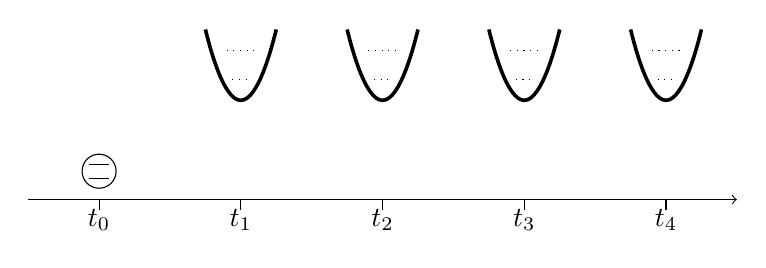
\begin{tikzpicture}[xscale=1.8, yscale=1.8]
      %% Axis and oscillators
      \draw[->,color=black] (-0.5,-.2) -- (4.5,-.2);
      \draw[shift={(0,-0.2)}, color=black] (0pt,-2pt) -- (0pt,0pt) node[below] {$t_0$};
      \foreach \x in {1, 2, 3, 4}
      {%
        \draw[shift={(\x,-0.2)}, color=black] (0pt,-2pt) -- (0pt,0pt) node[below] {$t_\x$};
        \draw[line width=1.3pt] ({\x - 0.25}, 1) parabola bend (\x, 0.5) ({\x + 0.25}, 1);
        \draw[dotted,color=black] ({\x - 0.06}, 0.65) -- ({\x + 0.06}, 0.65);
        \draw[dotted,color=black] ({\x - 0.1}, 0.85) -- ({\x + 0.1}, 0.85);
      }

      %% Two level system
      \node (TL) at (0, 0) {};
      \draw (TL) ellipse (.12 and 0.12);
      \draw ($(TL) + (0.07,0.05)$) -- ($(TL) + (-0.07,0.05)$);
      \draw ($(TL) + (0.07,-0.05)$) -- ($(TL) + (-0.07,-0.05)$);

    \end{tikzpicture}
    \caption{At $t = t_0$ all time-oscillators are in their ground-state due to the vacuum initial conditions.}
    \label{fig:nmqsd.timeosz0}
  \end{subfigure}
  \vspace{1cm}

  \begin{subfigure}[t]{1\textwidth}
    \centering
    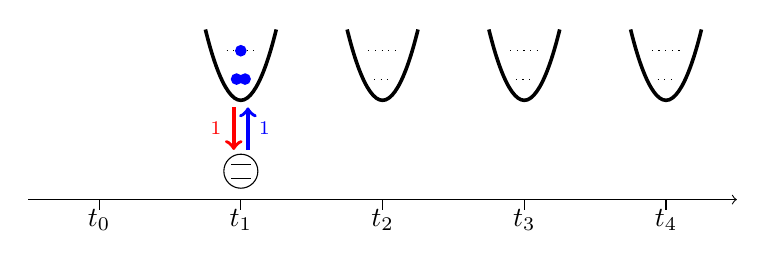
\begin{tikzpicture}[xscale=1.8, yscale=1.8]
      %% Axis and oscillators
      \draw[->,color=black] (-0.5,-.2) -- (4.5,-.2);
      \draw[shift={(0,-0.2)}, color=black] (0pt,-2pt) -- (0pt,0pt) node[below] {$t_0$};
      \foreach \x in {1, 2, 3, 4}
      {%
        \draw[shift={(\x,-0.2)}, color=black] (0pt,-2pt) -- (0pt,0pt) node[below] {$t_\x$};
        \draw[line width=1.3pt] ({\x - 0.25}, 1) parabola bend (\x, 0.5) ({\x + 0.25}, 1);
        \draw[dotted,color=black] ({\x - 0.06}, 0.65) -- ({\x + 0.06}, 0.65);
        \draw[dotted,color=black] ({\x - 0.1}, 0.85) -- ({\x + 0.1}, 0.85);
      }

      \draw[color=blue, line width=2pt] (1 - 0.03, 0.65) circle (0.02);
      \draw[color=blue, line width=2pt] (1 + 0.03, 0.65) circle (0.02);
      \draw[color=blue, line width=2pt] (1 + 0.0, 0.85) circle (0.02);

      %% Two level system
      \node (TL) at (1, 0) {};
      \draw (TL) ellipse (.12 and 0.12);
      \draw ($(TL) + (0.07,0.05)$) -- ($(TL) + (-0.07,0.05)$);
      \draw ($(TL) + (0.07,-0.05)$) -- ($(TL) + (-0.07,-0.05)$);

      \draw[->, color=blue, line width=1.3pt] ($(TL) + (0.05,0.15)$) -- node [right] {$\ZZ_1$} ++ (0, 0.3);
      \draw[<-, color=red, line width=1.3pt] ($(TL) + (-0.05,0.15)$) -- node [left] {$\adjZZ_1$} ++ (0, 0.3);

    \end{tikzpicture}
    \caption{%
      At $t = t_1$, the system interacts with the first time-oscillator, which is left in an excited state due to dissipated energy from the system.
      Since the remaining environment is still in its ground-state, the interaction via $\adjZZ_1$ is restricted to the first time-oscillator as well.
    }
    \label{fig:nmqsd.timeosz1}
  \end{subfigure}
  \vspace{1cm}

  \begin{subfigure}[t]{1\textwidth}
    \centering
    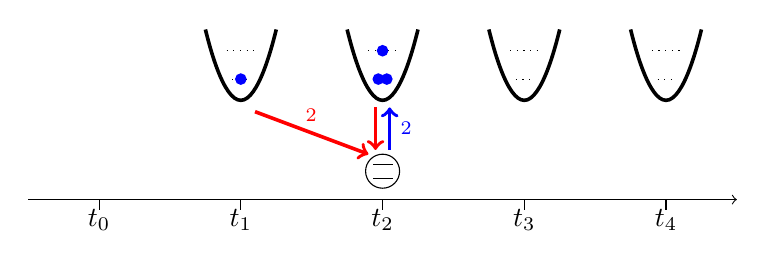
\begin{tikzpicture}[xscale=1.8, yscale=1.8]
      %% Axis and oscillators
      \draw[->,color=black] (-0.5,-.2) -- (4.5,-.2);
      \draw[shift={(0,-0.2)}, color=black] (0pt,-2pt) -- (0pt,0pt) node[below] {$t_0$};
      \foreach \x in {1, 2, 3, 4}
      {%
        \draw[shift={(\x,-0.2)}, color=black] (0pt,-2pt) -- (0pt,0pt) node[below] {$t_\x$};
        \draw[line width=1.3pt] ({\x - 0.25}, 1) parabola bend (\x, 0.5) ({\x + 0.25}, 1);
        \draw[dotted,color=black] ({\x - 0.06}, 0.65) -- ({\x + 0.06}, 0.65);
        \draw[dotted,color=black] ({\x - 0.1}, 0.85) -- ({\x + 0.1}, 0.85);
      }

      \draw[color=blue, line width=2pt] (1, 0.65) circle (0.02);
      \draw[color=blue, line width=2pt] (2 - 0.03, 0.65) circle (0.02);
      \draw[color=blue, line width=2pt] (2 + 0.03, 0.65) circle (0.02);
      \draw[color=blue, line width=2pt] (2 + 0.0, 0.85) circle (0.02);

      %% Two level system
      \node (TL) at (2, 0) {};
      \draw (TL) ellipse (.12 and 0.12);
      \draw ($(TL) + (0.07,0.05)$) -- ($(TL) + (-0.07,0.05)$);
      \draw ($(TL) + (0.07,-0.05)$) -- ($(TL) + (-0.07,-0.05)$);

      \draw[->, color=blue, line width=1.3pt] ($(TL) + (0.05,0.15)$) -- node [right] {$\ZZ_2$} ++ (0, 0.3);
      \draw[<-, color=red, line width=1.3pt] ($(TL) + (-0.05,0.15)$) -- node [left] {} ++ (0, 0.3);
      \draw[<-, color=red, line width=1.3pt] ($(TL) + (-0.1,0.12)$) -- node [above] {$\adjZZ_2$} ++ (-.8, 0.3);

    \end{tikzpicture}
    \caption{%
      For the next step $t = t_2$, the excitation of the bath is time-local as well---in general, the creation operator $\ZZ_n$ only changes the state of the single time-oscillator $t_n$.
      However, memory effects arise due to the feedback of the environment: $\adjZZ_2$ receives contributions from both preceding time steps, unless the weight-factor $\alpha_{1}$ vanishes.
    }
    \label{fig:nmqsd.timeosz2}
  \end{subfigure}
  \vspace{.5cm}

  \caption{%
    Pictorial interpretation of the time evolution described by the {\NMSSE}.
    The circle with two lines represents the system, while the harmonic potentials identify various time-oscillators.
  }
  \label{fig:nmqsd.timeosz}
\end{figure}
%%%%%%%%%%%%%%%%%%%%%%%%%%%%%%%%%%%%%%%%%%%%%%%%%%%%%%%%%%%%%%%%%%%%%%%%%%%%%%%%

Remarkably, the environmental operators in the full Hamiltonian~\ref{eq:nmqsd.Htot_time}, namely multiplication by $\ZZ_t$ and $\adjZZ_t$, have a simple interpretation in this picture:
The former simply acts as a creation operator for the time-oscillator-mode $t$ exactly as multiplication by $\cc z_\lambda$ acts as a creation operator for the physical oscillator-mode $\lambda$.
Of course, in the coherent state representation the corresponding annihilation operator is given by $\partial_{\cc z_\lambda}$.
The connection to the time-oscillator picture is most clearly explained using the expansion~\ref{eq:nmqsd.power_series} yielding
\begin{equation*}
  \partial_{\cc z_\lambda} \psi_t(\cc\zz) = \sum_{K=1}^\infty \left( \sum_{\lambda_1,\ldots,\lambda_{K-1}=1}^N K\, \psi_t^{(K)}(\lambda_1,\ldots\lambda_{K-1}, \lambda) \, \cc z_{\lambda_1} \ldots \cc z_{\lambda_{K-1}} \right),
\end{equation*}
where we use the symmetry of $\psi_t^{(K)}(\lambda_1, \ldots, \lambda_K)$ under permutation of the arguments and the independence-condition $\partial_{\cc z_\lambda} \cc z_\mu = \delta_{\lambda, \mu}$.
Similarly, annihilating an excitation of the time-oscillator mode $s$ for $0 < s < t$ in \autoref{eq:nmqsd.time_series} is achieved using the functional derivative
\begin{equation*}
  \frac{\delta \psi_t(\ZZ)}{\delta \ZZ_s} = \sum_K \intl{0}{t}{t_1} \ldots \intl{0}{t}{t_{K-1}} \, K \, \psi^{(K)}(t_1, \ldots, t_{K-1}, s) \, \ZZ_{t_1} \ldots \ZZ_{t_{K-1}},
\end{equation*}
since it satisfies the continuum independence-condition $\frac{\delta \ZZ_s}{\delta \ZZ_t} = \delta(t - s)$.

However, there is an important difference to the true bosonic ladder-operators:
As the microscopic definition~\ref{eq:nmqsd.stochastic_process} implies, the adjoint operator\footnote{%% FOOTNOTE
  Since the scalar-product in the full system-bath Hilbert space is given by
  \begin{equation*}
    \braket{\Psi}{\Phi} = \int \frac{\mathrm{d}^{2N} z}{\pi^N} \, \exp[-\abs{\zz}^2] \braket{\psi(\cc\zz)}{\phi(\cc\zz)} = \E[\braket{\psi(\ZZ)}{\phi(\ZZ)}],
  \end{equation*}
  this is exactly the statement of Novikov's formula~\ref{eq:nmqsd.novikov} with $P_t$ replaced by $\braket{\psi(\ZZ)}{\phi(\ZZ)}$.
}
of multiplication by $\ZZ_t$ is not the derivation $\frac{\delta}{\delta \ZZ_t}$, but $\adjZZ_t = \int \mathrm{d}s \, \alpha(t - s) \, \frac{\delta}{\delta \ZZ_s}$.
In other words, although we interpret $\ZZ_t$ as a creation operator of a time-oscillator mode $t$, the corresponding adjoint operator $\adjZZ_t$ does not simply annihilate an excitation of the same mode, but of all modes $s$ weighted by the correlation function $\alpha(t-s)$.\\



To explain the related interpretation of the \NMSSE more clearly, we switch to a discrete time step $\Delta t$ and set $t_n = n \Delta t$.
We introduce the corresponding time-discrete \quotes{process} $\ZZ_n = \frac{1}{\Delta t} \int_{t_{n-1}}^{t_n} \ZZ_t \dd t$ and the derivation operator $\adjZZ_n = \sum_k \alpha_{n-k} \, \partial_{\ZZ_k}$ in \autoref{cha:timeo}.
This allows us to approximate the time evolution for one step as
\begin{align*}
  \psi_{t_n}(\ZZ) = \exp[\Delta t (L \ZZ_n - \adj{L} \adjZZ_n)] \, \exp[-\ii \Delta t \Hsys] \, \psi_{t_{n-1}},
\end{align*}
with a free evolution of the system followed by an interaction with the time-oscillators---see \autoref{cha:timeo} for the details.
Already \autoref{fig:nmqsd.timeosz} displays the basic structure of the interaction
\begin{equation*}
  L \ZZ_n - \adj{L} \adjZZ_n = L \ZZ_n - \adj{L} \sum_k \alpha_{n - k} \, \frac{\partial}{\partial \ZZ_k}.
\end{equation*}
Since the creation operator $\ZZ_n$ involves only a single time-oscillator, the latter receive an excitation only once during the time evolution.
In contrast, the annihilation operators $\partial_{\ZZ_k}$ appear in each time step weighted by the bath-correlation function $\alpha_{n-k}$.
Except for the Markov limit $\alpha_{n-k} = \gamma\delta_{nk}$, memory effects arise by coupling to previously excited time-oscillators.
Of course, such a causal interpretation works only for an initial vacuum state of the environment.
If $\partial_{\ZZ_k} \psi_0 \neq 0$, we get contributions to $\adjZZ_n$ from all initially excited time-oscillators and therefore, the interpretation does not correspond to the common picture of an \quotes{environment with memory}.


%%%%%%%%%%%%%%%%%%%%%%%%%%%%%%%%%%%%%%%%%%%%%%%%%%%%%%%%%%%%%%%%%%%%%%%%%%%%%%%
\section{Finite Temperature Theory}
\label{sec:nmqsd.temperature}
% * why necessary
% * why approach does not work anymore
%
%%%%%%%%%%%%%%%%%%%%%%%%%%%%%%%%%%%%%%%%%%%%%%%%%%%%%%%%%%%%%%%%%%%%%%%%%%%%%%%

Until now, we were only concerned with the zero temperature theory, which is characterized by an initial product $\ket{\Psi_0} = \ket{\psi_0} \otimes \ket{\vec 0}$ with the environment in the vacuum state.
It translates into our \NMSSE-framework as the demand of vanishing functional derivatives $\frac{\delta \psi_0}{\delta \ZZ_s} = 0$ for arbitrary $s$.
This property ensures the bounded integral domain of $\adjZZ_t = \int\mathrm{d}s \, \alpha(t-s) \frac{\delta}{\delta \ZZ_s}$, which on the other hand is crucial for a causal interpretation in terms of time-oscillators.
Also, the $O$-operator substitution as well as the hierarchical equations of motion depend on the temperature-zero assumption.
In order to treat a thermal environment at arbitrary temperature, we present a method that maps to the vacuum initial conditions.

Let us consider an initial product, where the bath is described by a Gibbs state $\rho(\beta) = Z^{-1} \, \exp[-\beta \Henv]$; more precisely
\begin{equation}
  \rho_0 = \ket{\psi_0}\bra{\psi_0} \otimes \rho(\beta),
  \label{eq:nmqsd.initial_rho}
\end{equation}
with the bath partition function $Z = \Tr \exp[-\beta \Henv]$ at inverse temperature $\beta = T^{-1}$.
However, we cannot drop the requirement of separability for the initial state.\\



The thermo-field approach \cite{SeUm83_thermofield} is based on the simple trick that a thermal state $\rho(\beta)$ can be expressed as vacuum in an enlarged environment, doubling the degrees of freedom.
It is favored over other methods in the application to the \NMSSE since it preserves its structure.
Additionally, it constitutes a consistent way to include negative frequency oscillators in the environment, which on the other hand are required for the bath correlation function used to derive our hierarchy.
The last point is further elaborated in \autoref{sec:num.expansion}.
In the course of this section we follow the more detailed accounts of Yu and Strunz \cite{Yu04_heat_bath,St01_habil}.

The main idea is to introduce a second fictitious bath of oscillators $\mathcal{B}$, which is independent from the physical environment $\mathcal{A}$ and does not interact with the system.
Expressing its degrees of freedom in ladder operators $b_\lambda$ and $\adj{b}_\lambda$ yields the new Hamiltonian in the Schrödinger picture
\begin{equation}
  \Htot = \Hsys \otimes \unit + \sum_\lambda (\cc{g}_\lambda L\otimes\adj{a}_\lambda + g_\lambda \adj{L}\otimes a_\lambda) + \unit \otimes \sum_\lambda \omega_\lambda (\adj{a}_\lambda a_\lambda - \adj{b}_\lambda b_\lambda).
  \label{eq:nmqsd.Htot_thermal}
\end{equation}
Although the corresponding eigen-energies are not bounded from below due to negative frequencies of the fictitious oscillators, there are no stability problems since the latter do not interact with the physical degrees of freedom.
For the same reason, the reduced time evolution obtained from \autoref{eq:nmqsd.Htot_thermal} is identical to the original microscopic model~\ref{eq:nmqsd.Htot}.
Both yield equal reduced density matrices provided we choose an initial state $\tilde\rho$ for environments $\mathcal{A}$ and $\mathcal{B}$ that reproduces the environmental state in \autoref{eq:nmqsd.initial_rho} after tracing over the unphysical degrees of freedom, that is
\begin{equation}
  \Tr_\mathcal{B} \tilde\rho = \rho(\beta).
  \label{eq:nmqsd.rho_tilde}
\end{equation}
Here, $\Tr_\mathcal{B}$ denotes the partial trace with respect to the fictitious degrees of freedom.

Remarkably, a solution $\tilde\rho$ of \autoref{eq:nmqsd.rho_tilde} is given by a pure state projector on a vacuum state with respect to new annihilation operators $A$, $B$.
They are connected to the old ladder operators by a temperature dependent \emph{Bogoliubov transformation}
\begin{align*}
  A_\lambda &= \sqrt{\bar n_\lambda + 1} \, a_\lambda + \sqrt{\bar n_\lambda} \, \adj{b}_\lambda \\
  B_\lambda &= \sqrt{\bar n_\lambda} \, \adj{a}_\lambda + \sqrt{\bar n_\lambda + 1} \, b_\lambda,
\end{align*}
with $\bar n_\lambda = \left( \exp(\beta \omega_\lambda) - 1 \right)^{-1}$ denoting the mean thermal occupation number of the (physical) oscillator mode $\lambda$.
An extensive but elementary calculation reveals that $\tilde\rho = \ket{0_{AB}}\bra{0_{AB}}$ with $\ket{0_{AB}} = \ket{0_A} \otimes \ket{0_B}$ satisfies \autoref{eq:nmqsd.rho_tilde} \cite{SeUm83_thermofield}.
The doubling in degrees of freedom ensures that the reduced density matrix obtained from an initial pure state $\ket{\tilde\Psi_0} = \ket{\psi_0}\otimes\ket{0_{AB}}$ in the enlarged Hilbert space coincides with the original state at finite temperature~\ref{eq:nmqsd.initial_rho}.
Expressed in these new coordinates the total Hamiltonian~\ref{eq:nmqsd.Htot_thermal} reads
\begin{align}
  \Htot = \Hsys\otimes\unit &+ \sum_\lambda \sqrt{\bar n_\lambda + 1} \, \left(\cc g_\lambda L\otimes\adj{A}_\lambda + g_\lambda \adj{L}\otimes A_\lambda \right) \nonumber \\
        \label{eq:nmqsd.Htot_thermal_shifted}
        &+ \sum_\lambda \sqrt{\bar n_\lambda} \, \left( g_\lambda \adj{L}\otimes\adj{B}_\lambda  + \cc g_\lambda L \otimes B_\lambda \right) \\
        &+ \unit \otimes \sum_\lambda \omega_\lambda \left( \adj{A}_\lambda A_\lambda - \adj{B}_\lambda B_\lambda \right). \nonumber
\end{align}
This is identical to the zero temperature model, except now the system is coupled to two separate harmonic baths instead of one.
Therefore, we need two independent processes $\ZZ_t$ and $\cc{W}_t$ for a stochastic version of \autoref{eq:nmqsd.Htot_thermal_shifted} in general:
\begin{align}
  \partial_t \psi_t = -\ii\Hsys\psi_t &+ L\ZZ_t\psi_t - \adj{L}\int_0^t \alpha_1(t-s) \frac{\delta \psi_t}{\delta \ZZ_s} \dd s \nonumber \\
  &+ \adj{L} \cc{W}_t \psi_t - L\int_0^t \alpha_2(t-s) \frac{\delta\psi_t}{\delta \cc{W}_s} \dd s.
  \label{eq:nmqsd.nmsse_thermal_2processes}
\end{align}
All effects of the original thermal initial state are now encoded in the correlation functions
\begin{equation}
  \alpha_1(t) = \sum_\lambda (\bar n_\lambda + 1) \abs{g_\lambda}^2 \exp[-\ii\omega_\lambda t] \quad \mbox{and} \quad
  \alpha_2(t) = \sum_\lambda \bar n_\lambda \abs{g_\lambda}^2 \exp[\ii\omega_\lambda t]
  \label{eq:nmqsd.cov_2processes}
\end{equation}
for $\ZZ_t$ and $\cc{W}_t$ respectively.
Both are Gaussian, thus independence of $\ZZ$ and $\cc W$ is equivalent to vanishing mutual covariance $\E[\ZZ_t W_s] = \E[Z_t W_s] = 0$.

As we doubled the bath degrees of freedom merely to cope with a thermal initial state, it is quite natural that the zero-temperature result~\ref{eq:nmqsd.nmsse} with a single noise process is recovered in the limit $T \to 0$:
With vanishing occupation numbers $n_\lambda \to 0$ both, $\alpha_2$ and $\cc W_t$, go to zero, while $\alpha_1$ reproduces the original bath correlation function~\ref{eq:nmqsd.correlation_function}.

The thermo-field approach is especially simple for a self-adjoint coupling operator $L = \adj{L}$.
Indeed, we can combine both processes in \autoref{eq:nmqsd.nmsse_thermal_2processes} into a single one, which we denote by $\tildeZZ_t \ZZ_t + \cc W_t$.
Since $\ZZ$ and $\cc W$ are mutual independent by assumption and $2\bar n_\lambda + 1 = \coth{\frac{\beta\omega_\lambda}{2}}$, we find for the crucial correlation function
\begin{equation}
  \E[\tilde Z_t \tildeZZ_s] = \sum_\lambda \left(\abs{g_\lambda}^2 \, \coth{\frac{\beta \omega_\lambda}{2}} \, \cos{\omega_\lambda (t-s)} - \ii \sin{\omega_\lambda (t-s)} \right).
  \label{eq:nmqsd.combined_correlation}
\end{equation}
Consequently, the finite temperature \NMSSE with self-adjoint coupling operators is identical to the $T=0$ version except for a modified correlation function.
It is not surprising that the combined correlation function~\ref{eq:nmqsd.combined_correlation} agrees with the result of Feynman and Vernon already encountered in \autoref{eq:nmqsd.thermal_correlation_function}, which is usually derived by means of path integration \cite{FeVe63_quantum_dissipative}.
But the approach presented here is much more general since it can tackle any kind of open quantum system with linear coupling.

%%%%%%%%%%%%%%%%%%%%%%%%%%%%%%%%%%%%%%%%%%%%%%%%%%%%%%%%%%%%%%%%%%%%%%%%%%%%%%%%
%\subsection{unitary noise}
%\label{sub:nmqsd.temperature.unitary}
%% * method
%% * would be better for hierarchies
%% * still negative energies
%% * problematic integral
%% * classical noise --> alpha purely real

%As shown in the last section we can treat classical thermal noise on the same footing as quantum noise under certain circumstances just by using a modified correlation function~\ref{eq:nmqsd.combined_correlation}.
%It is worth noticing how the influence of thermal fluctuations modify only the real part of $\alpha$, a feature that explicitly distinguishes noisy classical perturbations \cite{FeHi10_path_integrals}.
%Therefore it is quite instructive to present a different method for treating non-zero temperature within the non-Markovian quantum state diffusion.

%We start off by expanding the thermal bath state in a coherent state basis \cite{WaMi08_quantum_optics}
%\begin{equation*}
  %\rho(\beta) = FILL IN
%\end{equation*}
%which is quite reminiscent of the expansion for a pure state projector that lead to our stochastic Schrödinger equation.
%The corresponding pure initial states are a product involving all environmental oscillators
%\begin{equation*}
  %\ket{\Psi_0(\xi)} = \exp[-\frac{\abs{\vec\xi}^2}{2}] \ket{\psi_0} \bigotimes_\lambda \ket{\xi_\lambda}
%\end{equation*}
%where the additional prefactor is usually absorbed by using normalized coherent states.
%A simple shift for the creation and annihilation operators $\adj{A}_\lambda = \adj{a}_\lambda - \cc{\xi}_\lambda$ and $A_\lambda = a_\lambda - \xi_\lambda$ respectively maps the environmental part of the initial state above onto the vacuum.
%Therefore we can apply our zero-temperature derivation to the total Hamiltonian expressed in $A$ and $\adj{A}_\lambda$.
%The resulting \NMSSE reads
%\begin{equation}
  %\partial_t \psi_t(\ZZ, \xi) = \left( -\ii\Hsys + L\cc\xi_t + \adj{L}\xi_t + L\ZZ_t - \adj{L}\int_0^t \alpha(t - s) \frac{\delta}{\delta \ZZ_s} \dd s \right) \psi_t(\ZZ, \xi, \cc\xi)
  %\label{eq:nmqsd.nmsse_thermal_classic}
%\end{equation}
%with a classical driving process $\xi_t = \sum_\lambda g_\lambda \xi_\lambda \exp[-\ii \omega_\lambda t]$ and its familiar quantum counterpart $\ZZ_t$.
%The former's properties are once again fixed by its correlations
%\begin{equation*}
  %\E\,\xi_t = 0, \quad \E\,\xi_t \xi_s =0, \quad\mbox{and}\quad \E\,\xi_t \cc{\xi}_s = 2\sum_\lambda \bar n_\lambda \abs{g_\lambda}^2 \cos{\omega_\lambda(t-s)}.
  %\label{eq:nmqsd.process_properties}
%\end{equation*}
%%Recovering the reduced density matrix not only requires an average over $\ZZ$ but also over all realizations of the thermal noise process $\xi_t$.
%Since all thermal occupation numbers $\bar n_\lambda$ tend to zero for $T \to 0$, we obtain the zero temperature limit simply by setting $\xi_t = 0$.
%This amounts to the trivial decomposition $\rho(T = 0) = \ket{\vec 0}\bra{\vec 0}$ of the zero temperature environmental state.

%%%%%%%%%%%%%%%%%%%%%%%%%%%%%%%%%%%%%%%%%%%%%%%%%%%%%%%%%%%%%%%%%%%%%%%%%%%%%%%
\section{Jaynes-Cummings Model}
\label{sec:nmqsd.two_level}
%%%%%%%%%%%%%%%%%%%%%%%%%%%%%%%%%%%%%%%%%%%%%%%%%%%%%%%%%%%%%%%%%%%%%%%%%%%%%%%

% ✔ originaly introduced to model decay of two-level atom coupled to single mode of cavity; comparisson of semi-classical and quantized theory of radiation
% ✔ two level system H=σ_z; coupled to possibly structured environment; dipol approximation
% ✔ far-off resonance for other levels of atom --> effective two level system
% * here general spectral density
%
The Jaynes-Cummings model was originally introduced to study the decay of an atom coupled to a single quantized mode of the electro-magnetic field in a cavity \cite{JaCu63_radiation_theory}.
It describes a single electronic excitation of the atom with energy $\omega$ above ground state in terms of an effective two level system with $\Hsys = \frac{\omega}{2}\sigma_z$.
Other electronic levels can be neglected safely, if their excitation energy is much larger than $\omega$ or far off-resonant compared to the cavity mode.
In dipole and rotating-wave approximation the system's coupling operator to the bath is $L = g\sigma_-$, therefore, the corresponding \NMSSE reads
\begin{equation}
  \partial_t \psitZ = -\ii\frac{\omega}{2}\sigma_z\psitZ + g \sigma_- \ZZ_t \psitZ - g\sigma_+ \int_0^t \alpha(t - s) \frac{\delta\psitZ}{\delta \ZZ_s} \dd s.
  \label{eq:nmqsd.nmsse_twolevel}
\end{equation}
supplied with initial conditions $\psi_0(\ZZ) = \psi_0$.
This approximation holds as long as the coupling strength $g$ is very small compared to the cavity transition frequency.
Only recently, experiments in circuit quantum electrodynamics detected effects from so called counter-rotating interaction terms \cite{NiDeHu10_circuit_qed}.
Here, we also cover the more general case of a possibly structured environment.

The Jaynes-Cummings model is a rare example, where an analytic solution for the $O$-operator is known \cite{DiGiSt98_nmqsd}, which we outline first.
Afterwards, we present a new solution-strategy, which is more in the spirit of this work, and discuss a possible problem of the $O$-operator substitution in numerical calculations.


%%%%%%%%%%%%%%%%%%%%%%%%%%%%%%%%%%%%%%%%%%%%%%%%%%%%%%%%%%%%%%%%%%%%%%%%%%%%%%%
\subsection{O-Operator Method}
\label{sub:nmqsd.two_level.o}
%

As elaborated in \autoref{sub:nmqsd.lin_nmsse.convolutionless} we can simplify the \NMSSE~\ref{eq:nmqsd.nmsse_twolevel} by replacing the functional derivative with an operator $O(t, s, \ZZ)$.
We try to solve the consistency condition~\ref{eq:nmqsd.consistency_condition} by a noise-independent ansatz \cite{DiGiSt98_nmqsd}
\begin{equation}
  O(t, s) = g f(t, s) \sigma_-.
  \label{eq:nmqsd.o_ansatz}
\end{equation}
Hence, all non-Markovian feedback from the environment is now encoded in the function $f(t, s)$ to be determined.
Plugging this ansatz into the evolution equation for $O(t,s)$ yields
\begin{equation}
  \partial_t f(t, s) \sigma_- = \left[-\ii \frac{\omega}{2} \sigma_z - g^2 F(t) \sigma_+\sigma_-, f(t, s) \sigma_-\right]
  \label{eq:nmqsd.eom_for_o}
\end{equation}
with the shorthand notation $F(t) := \int_0^t \alpha(t-s) f(t, s) \dd s$.
From its definition~\ref{eq:nmqsd.o_bar}, we see that $F(t)$ is also the coefficient of the integrated operator $\bar O(t) = g F(t) \sigma_-$.
Since the operator algebra in \autoref{eq:nmqsd.eom_for_o} closes, our ansatz solves the equation of motion for $O(t,s)$ provided $f(t,s)$ evolves according to
\begin{equation*}
  \partial_t f(t, s) = \left(\ii \omega + g^2 F(t)\right) \, f(t, s), \qquad 0 \le s \le t.
\end{equation*}
Appropriate initial conditions follow trivially from \autoref{eq:nmqsd.o_initial}, namely $f(s, s) = 1$.
In the special case of an exponential bath correlation function $\alpha(t) = \exp[-\gamma\abs{t} - \ii\Omega t]$ we can also derive a differential equation that is closed in $F$, namely
\begin{equation}
  \partial_t F(t) = 1 + (\ii (\omega - \Omega) - \gamma) F(t) + g^2 F(t)^2.
  \label{eq:nmqsd.twolevel_f}
\end{equation}
Such exponential correlation functions $\alpha(t) = \exp[-\gamma\abs{t} - \ii\Omega t]$ play a major role in the subsequent work.
Once $F$ is known, we can determine solutions of the convolutionless \NMSSE~\ref{eq:nmqsd.nmsse_o} for given noise realizations or---since $O$ is independent of $\ZZ$---directly calculate the reduced density operator using the master equation~\ref{eq:nmqsd.master}.

%%%%%%%%%%%%%%%%%%%%%%%%%%%%%%%%%%%%%%%%%%%%%%%%%%%%%%%%%%%%%%%%%%%%%%%%%%%%%%%
\subsection{Noise-Expansion Method}
\label{sub:nmqsd.expansion}

In this section we propose a different approach to \autoref{eq:nmqsd.nmsse_twolevel}.
It is based on the expansion discussed in \autoref{sec:nmqsd.interpretation}, which allows us to express the quantum trajectories $\psitZ$ in a functional Taylor series with respect to the noise process
\begin{equation*}
  \psitZ = \twovec{\psi^+(t)}{\psi^-(t)} + \int_0^t \twovec{\psi^+_s(t)}{\psi^-_s(t)} \ZZ_s \dd s.
\end{equation*}
Due to the particular coupling structure of the model we make an ansatz at most linear it $\ZZ_t$.
As further elaborated in \autoref{sec:tla.general} our \NMSSE~\ref{eq:nmqsd.nmsse_twolevel} reduces to a $\Complex$-valued integro-differential equation
\begin{equation}
  \dot\psi^+(t) = -\ii \frac{\omega}{2} \psi^+(t) - g^2 \int_0^t \alpha(t - s) \exp[\ii \frac{\omega}{2} (t - s)] \psi^+(s) \dd s
  \label{eq:nmqsd.dotpsi_plus}
\end{equation}
with initial conditions $\psi^+(0) = \psi_0^+$, which is nevertheless quite involved---even from a numerical point of view.
Again, the situation simplifies dramatically for an exponential correlation function; the details are provided in \autoref{sec:tla.exp}.

Nevertheless, we may still discover some illuminating consequences concerning the $O$-operator without an explicit solution for $\psi^+(t)$.
With $\psi^-(t) = \psi^-_0 \, \exp(\ii \omega t / 2)$ the full quantum trajectory reads
\begin{equation}
  \psi_t(\ZZ) = \twovec{\psi^+(t)}{\psi^-(t)} + g \int_0^t \twovec{0}{\exp[\ii \frac{\omega}{2} (t-s)] \psi^+(s)} \ZZ_s \dd s.
  \label{eq:nmqsd.solution}
\end{equation}
This allows us to calculate the functional derivative with respect to the noise process explicitly; for $0 < s < t$ we find
\begin{equation*}
  \frac{\delta \psi_t(\ZZ)}{\delta \ZZ_s} = g \twovec{0}{\exp[\ii \frac{\omega}{2} (t-s)] \psi^+(s)},
\end{equation*}
which agrees with our ansatz~\ref{eq:nmqsd.o_ansatz} if we choose
\begin{equation}
  f(t, s) = \frac{\psi^+(s)}{\psi^+(t)} \, \exp[\ii \frac{\omega}{2}(t - s)].
  \label{eq:nmqsd.o_ansatz_psi}
\end{equation}
A similar structure for the $O$-operator has been obtained before using a Heisenberg-operator technique \cite{St01_habil}.\\

\begin{figure}
  \centering
  \includegraphics[width=\columnwidth]{img/jaynescummings.pdf}
  \caption{%
    Expectation value $\qmean{\sigma_z}$ for the Jaynes-Cummings model with an exponentially decaying bath correlation function $\alpha(t) = \frac{\gamma}{2} \exp[-\gamma\abs{t} - \ii\Omega t]$ in resonance ($\Omega = \omega$) and coupling strength $g = \sqrt{2}$ calculated using \autoref{eq:tla.solution}.
    Insets show $\vert F \vert$ representing magnitude of $\bar O$.
    \textbf{(A)} Strongly damped $\gamma = 4\omega$,
    \textbf{(B)} Weakly damped $\gamma = 0.1\omega$; the dashed line represent the same parameter set, but slightly moved off-resonance ($\Omega = 1.01\omega$).
  }
  \label{fig:nmqsd.jaynes_cummings}
\end{figure}

% * Discuss \bar O, here non-trivial part is F(t); relevant part in numerical application \cite
% * formula for \psi^+(t) (\sigma_z); sigma_z = -1 <==> psi^+ = 0 (from density operator + Tr ρ = 1)

Recall that the convolutionless \NMSSE of the last section reduces to a nonlinear differential equation~\ref{eq:nmqsd.twolevel_f} for
\begin{equation}
  F(t) = \int_0^t \alpha(t - s) \exp[\ii \frac{\omega}{2} (t - s)] \frac{\psi^+(s)}{\psi^+(t)} \dd s,
  \label{eq:nmqsd.twolevel_f_integral}
\end{equation}
where $f(t, s)$ has already been replaced by the expression~\ref{eq:nmqsd.o_ansatz_psi}.
We will now argue that it is exactly the denominator $\psi^+(t)$ that may cause problems in a numerical integration of~\ref{eq:nmqsd.twolevel_f}.
Indeed, calculating the reduced density matrix from \autoref{eq:nmqsd.solution} and using the condition $\Tr \rho_t = 1$, we find the connection $\qmean{\sigma_z}_{\rho_t} = 2\abs{\psi^+(t)}^2 - 1$.

% * already problematic in this simple model: <σ>_z --> -1 for t --> ∞; but also in between
%     => denominator in eq... problematic around psi^+(t) \approx 0 if
%        * alpha not decayed rapidly enough to cancel nonzero numerator
%        * or ψ^+_s approaches zero at t very steep
%     * figure show this behavior: if damping is large enough (A) no problem due to surpression by alpha
%     * (B) weak damping, decays on timescale tau = 10 => in that timescale below t=5, 15,... f(t, s) accumulates large contributions
%

Since for $\gamma \neq 0$ the atom described by the two-level system is expected to relax to its ground state, the denominator in~\ref{eq:nmqsd.twolevel_f_integral} eventually goes to zero.
Even worse are local extremal points $t_i$, where $\qmean{\sigma_z}_{\rho_t} \approx -1$, as we see in \autoref{fig:nmqsd.jaynes_cummings}:
The excitation in A decays almost exponentially due to the small memory time $\tau = \gamma^{-1}$ of the environment.
Therefore, $\frac{\psi^+(s)}{\psi^+(t)} \approx 1$ in the relevant time scale $s \in [t - \tau, t]$ of \autoref{eq:nmqsd.twolevel_f_integral}, so $\abs{F}$ approaches a constant value uniformly.
In contrast, the highly non-Markovian system B shows singular peaks in $\abs{F}$ for $\omega t \approx 5, 15$, where the expectation value of $\sigma_z$ is approximately $-1$.
These result from large fractions $\frac{\psi^+(s)}{\psi^+(t)}$, as the correlation function $\alpha(t-s)$ does not decay rapidly enough to suppress contributions in the integral with $\psi^+(s) \gg \psi^+(t)$.

% * resonance phenomenon: by small shift in ω, peaks much smaller
%     * cause: its not |ψ^+|, but ψ^+, for ω≠Ω cancelation in integral due to phase
% * since \bar O is only used to propagate \psi^+ ==> there large \bar O cancled by \psi^+(t);
%     => although differences of resonant and none-resonant in F huge, no differences in <σ_z>

These two different types of behavior for $\abs{F}$ are quite similar to the resonantly driven harmonic oscillator with strong or weak damping.
Also, notice how shifting the bath-frequency $\Omega$ only slightly off-resonance results in a much smoother $F$---as the dashed line in \autoref{fig:nmqsd.jaynes_cummings} B shows---while $\qmean{\sigma_z}$ remains virtually unchanged.
Actually, these large peaks do not contribute excessively to the end result, as they are canceled with the very small value of $\psi^+(t)$ in $\bar O(t) \psitZ$ (or in the corresponding master equation).
Still, the numerical solution of \autoref{eq:nmqsd.twolevel_f} requires a more careful treatment for the resonant case in order to correctly reproduce these peaks and not diverge to infinity.\\

% * not possible in real systems ==> more modes in bath, ZZ-dependent O
%     => more severe, densely spaced divergences known to appear in certain areas of parameter spaces, accumulate error
%     * exceed numerical accuracy
%     * supposed to be one reason for failure of O-operator calculation \cite private communication
% * better to propagate state to circumvent divergences ==> HiHiHiearchies!

Of course, all statements made in this section only hold for the simple Jaynes-Cummings model, and it is not clear, whether the $\bar O$-operator behaves similarly for more realistic systems.
Notwithstanding, an even more problematic behavior of $\max\limits_{m,n} \abs{\bar O_{mn}(t)}$, where $\bar O_{mn}(t)$ are the matrix elements of $\bar O(t)$ in the system-basis used, has been found in \textsc{ZOFE}-calculations for certain parameter regimes of more realistic systems\footnote{%
  Gerhard Ritschel, private communications.
  \textsc{ZOFE} stands for zero-order functional expansion and was introduced in \autoref{sub:nmqsd.lin_nmsse.convolutionless}.
}.
As for a larger number of bath modes resonances are more likely to occur, the situation is much more delicate in that case.
Likely, these numerical sophisticated problems are also responsible for divergences of higher order hierarchies in the $O$-operator making a systematic improvement of \textsc{ZOFE} quite involved.
We come to the conclusion that it can be advantageous to devise a numerical scheme in terms of the more regular $\bar O(t, \ZZ) \psitZ$ instead, as sharp contributions during the propagation might be smoothed away---this is exactly the approach used for our stochastic hierarchical equations of motion presented in the next chapter.
